\section{Experimental results}

\subsection{The single Fano cavity}

Figures:
\begin{itemize}
    \item Single fano cavity transmission as a function of wavelength.
    \item Short scan of the single fano cavity tranmission, with found linewidth.
    \item Long scan Fabry-Perot fringes for determining FSR -> cavity length. 
    \item linewidth as a function of cavity length (compare with broadban cavity).
\end{itemize}

\begin{figure}[h!]
    \centering
    \begin{subfigure}[b]{0.49\textwidth}
        \centering
        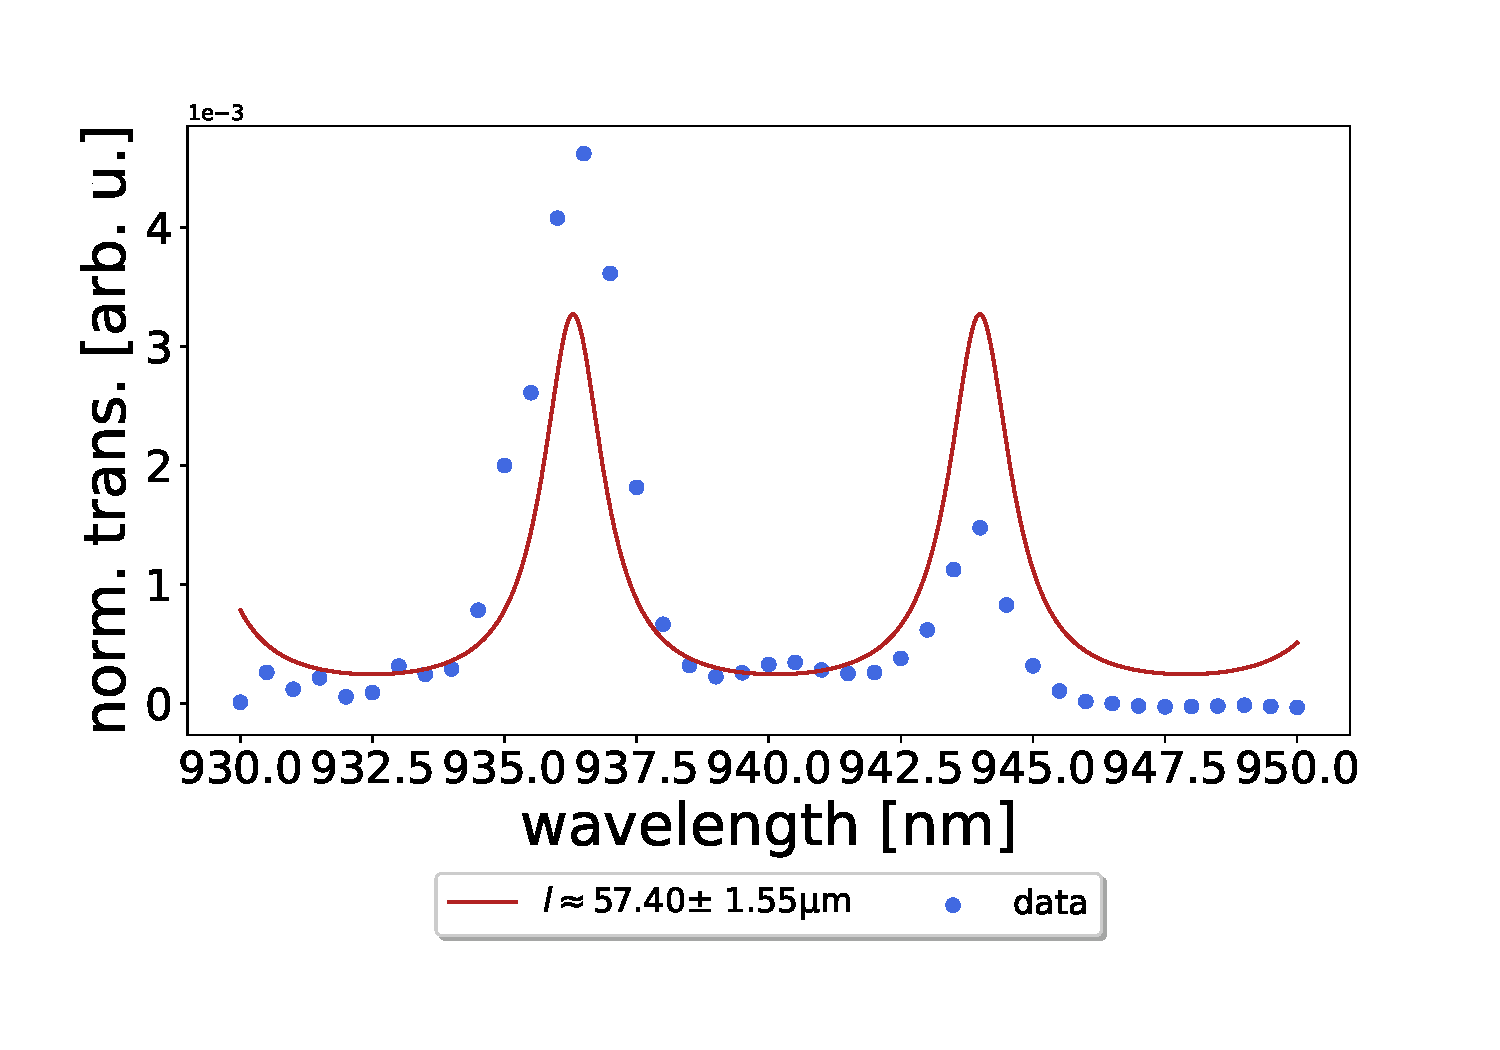
\includegraphics[width=\textwidth]{figures/results/60um_M5_FSR_fit.pdf}
        \caption{}
        \label{fig:short_single_fano_FSR}
    \end{subfigure}
    \begin{subfigure}[b]{0.49\textwidth}
        \centering
        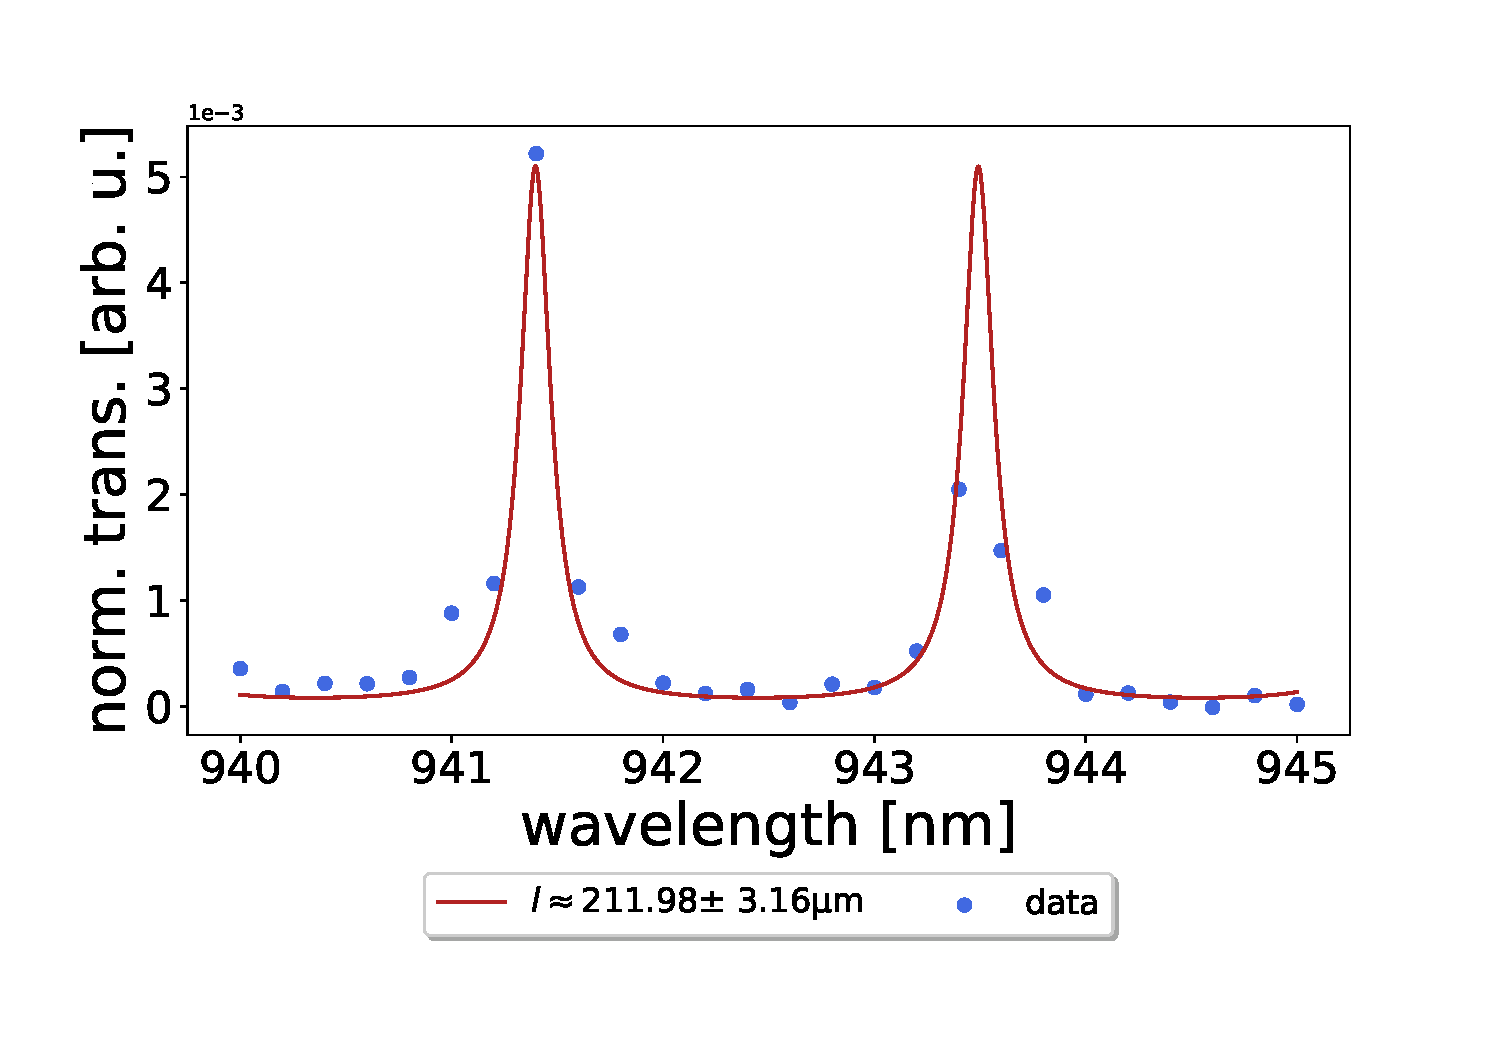
\includegraphics[width=\textwidth]{figures/results/220um_M5_FSR_fit.pdf}
        \caption{}
        \label{fig:long_single_fano_FSR}
    \end{subfigure}
\end{figure}

\begin{figure}[h!]
    \centering
    \begin{subfigure}[b]{0.49\textwidth}
        \centering
        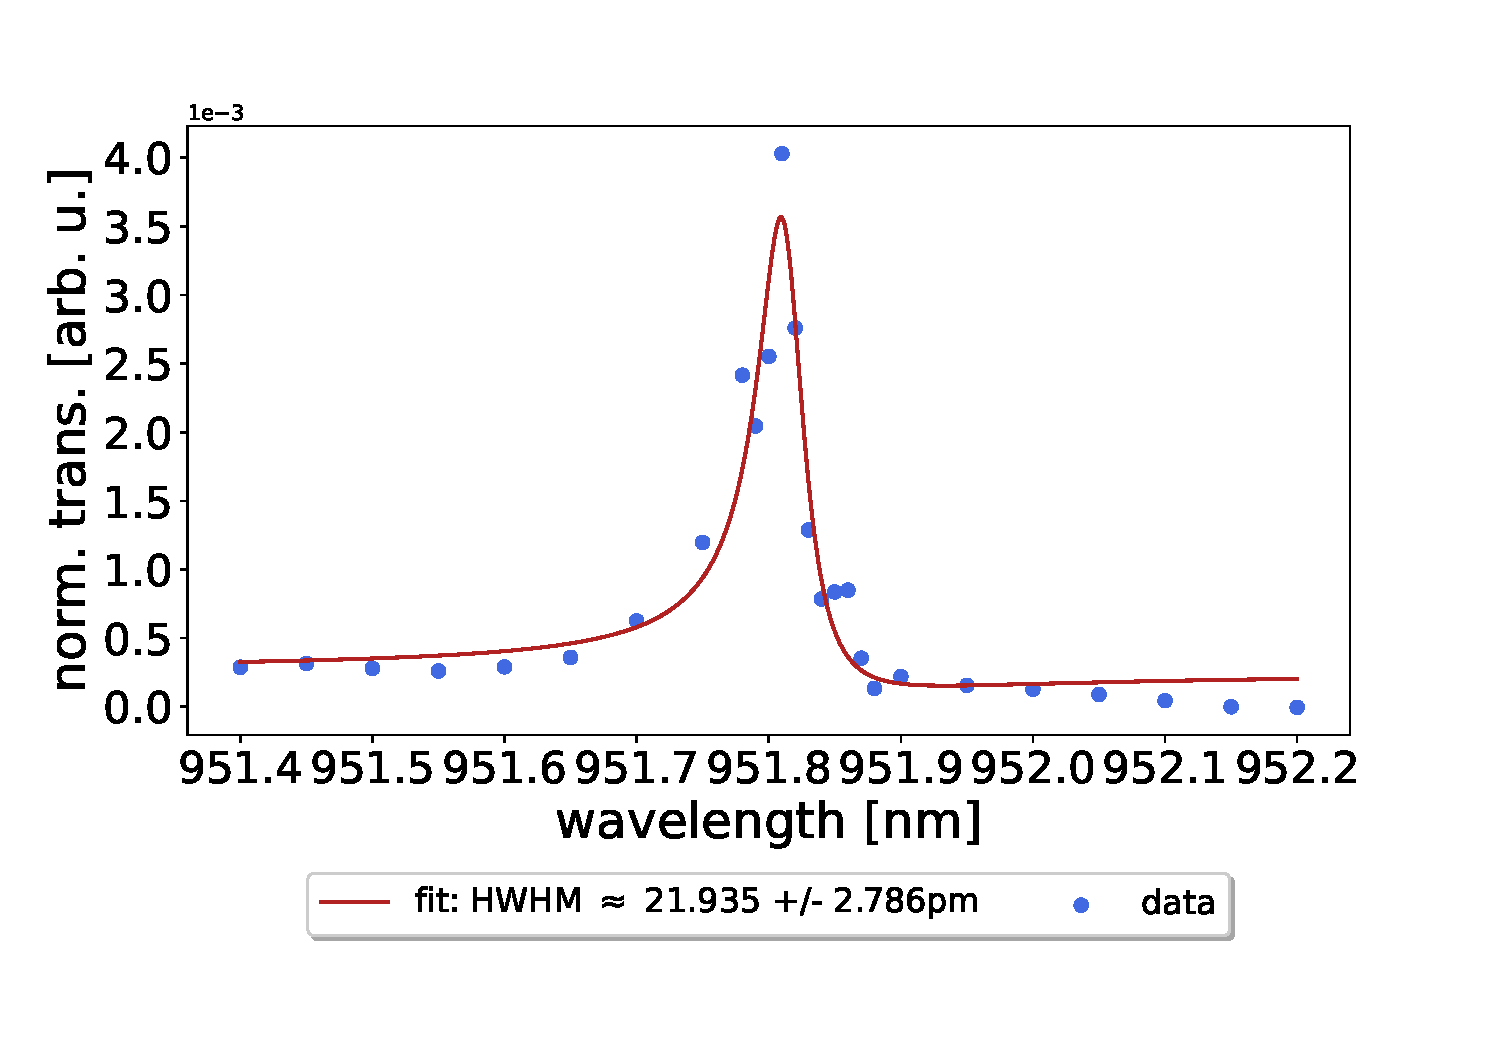
\includegraphics[width=\textwidth]{figures/results/60um_M5_fit_1.pdf}
        \caption{}
        \label{fig:short_single_fano_trans}
    \end{subfigure}
    \begin{subfigure}[b]{0.49\textwidth}
        \centering
        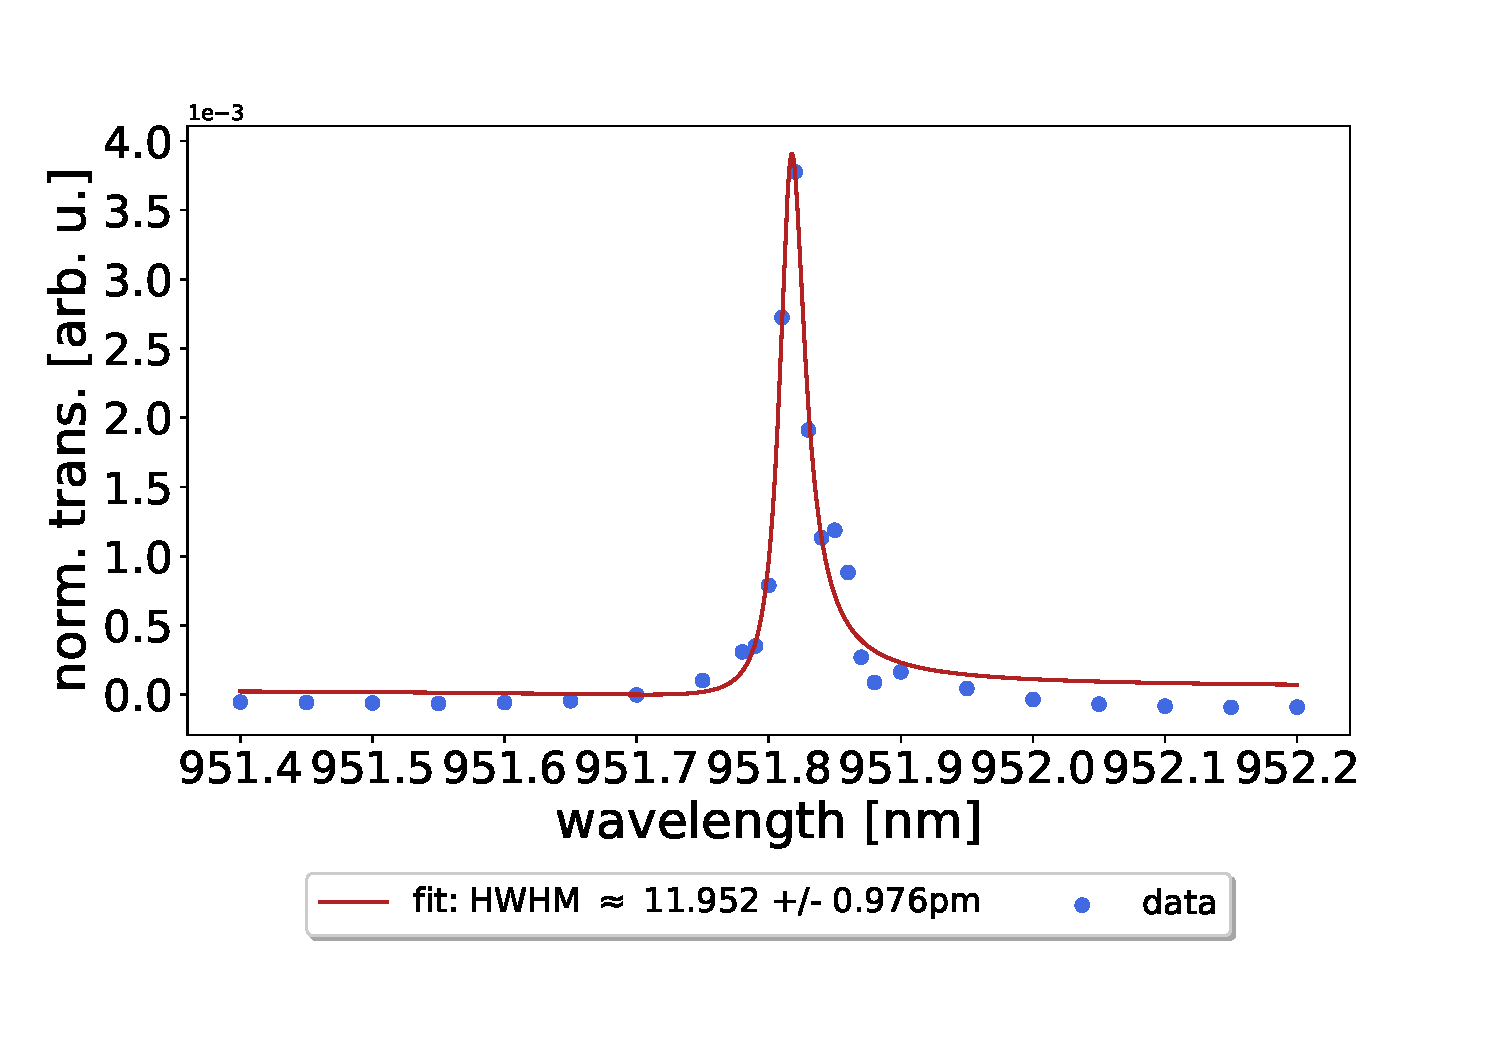
\includegraphics[width=\textwidth]{figures/results/220um_M5_fit_4.pdf}
        \caption{}
        \label{fig:long_single_fano_trans}
    \end{subfigure}
\end{figure}

\begin{figure}[h!]
    \centering
    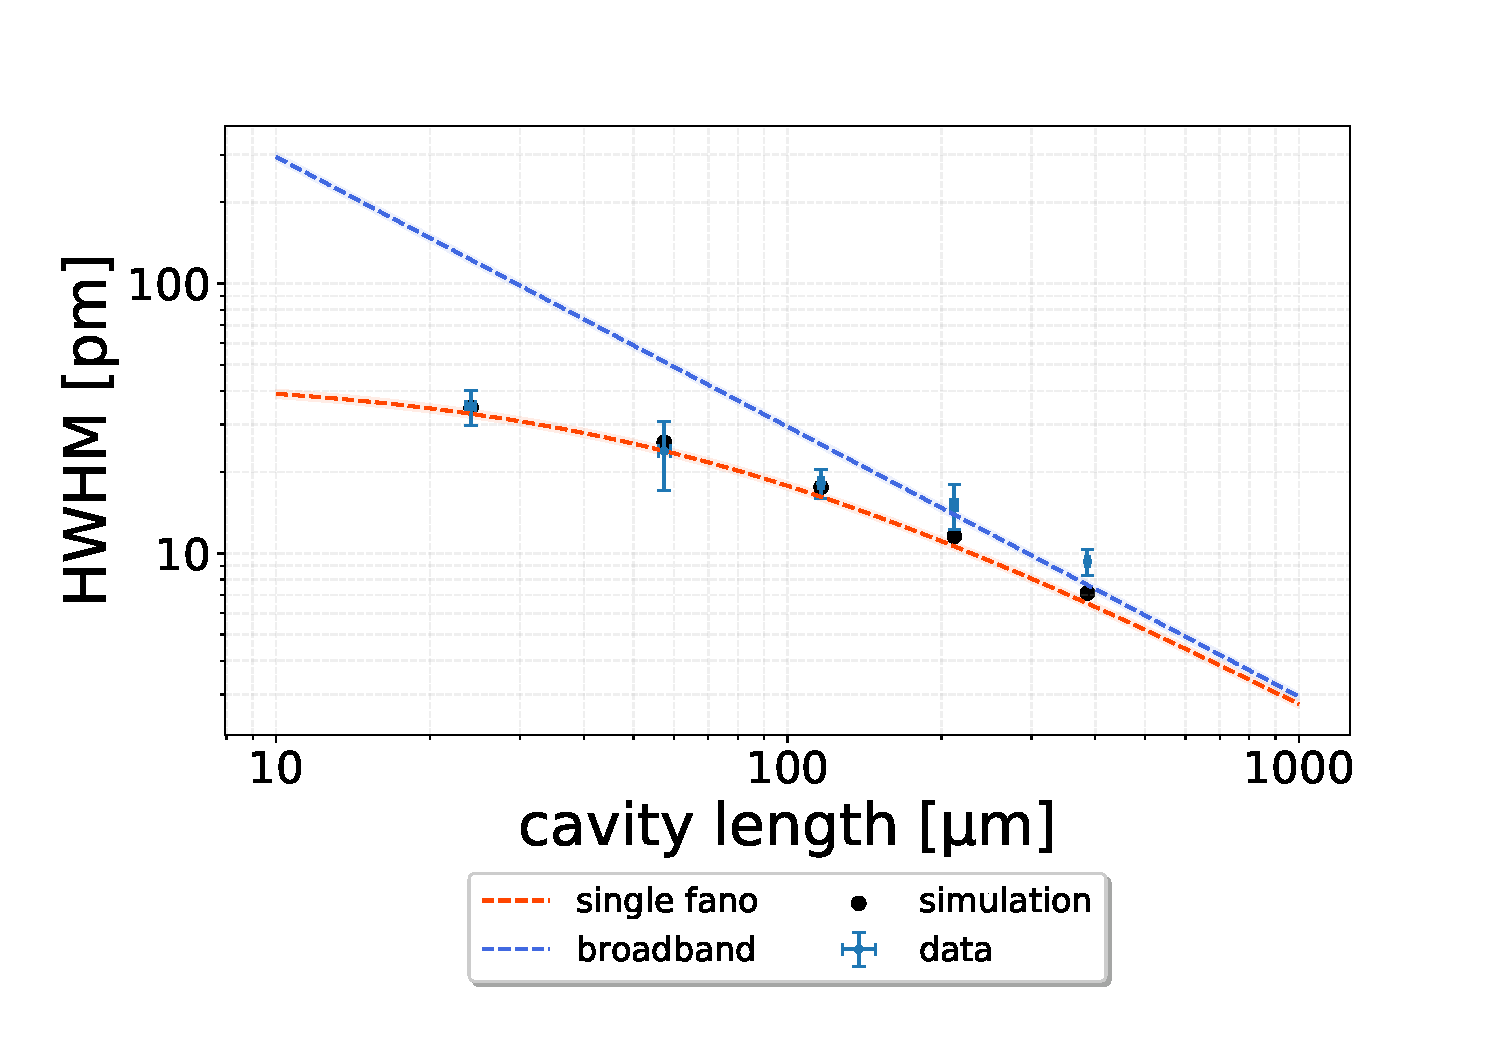
\includegraphics[width=0.7\textwidth]{figures/results/HWHM_vs_cavity_length_single_fano.pdf}
    \caption{}
    \label{fig:HWHM_vs_time_single_fano_data}
\end{figure}

\subsection{The double Fano cavity}

\subsubsection{Realizing the double fano model}

Figures: 
\begin{itemize}
    \item Fit of the double fano model (long + short cavity)
\end{itemize}

\begin{figure}[h!]
    \centering
    \begin{subfigure}[b]{0.49\textwidth}
        \centering
        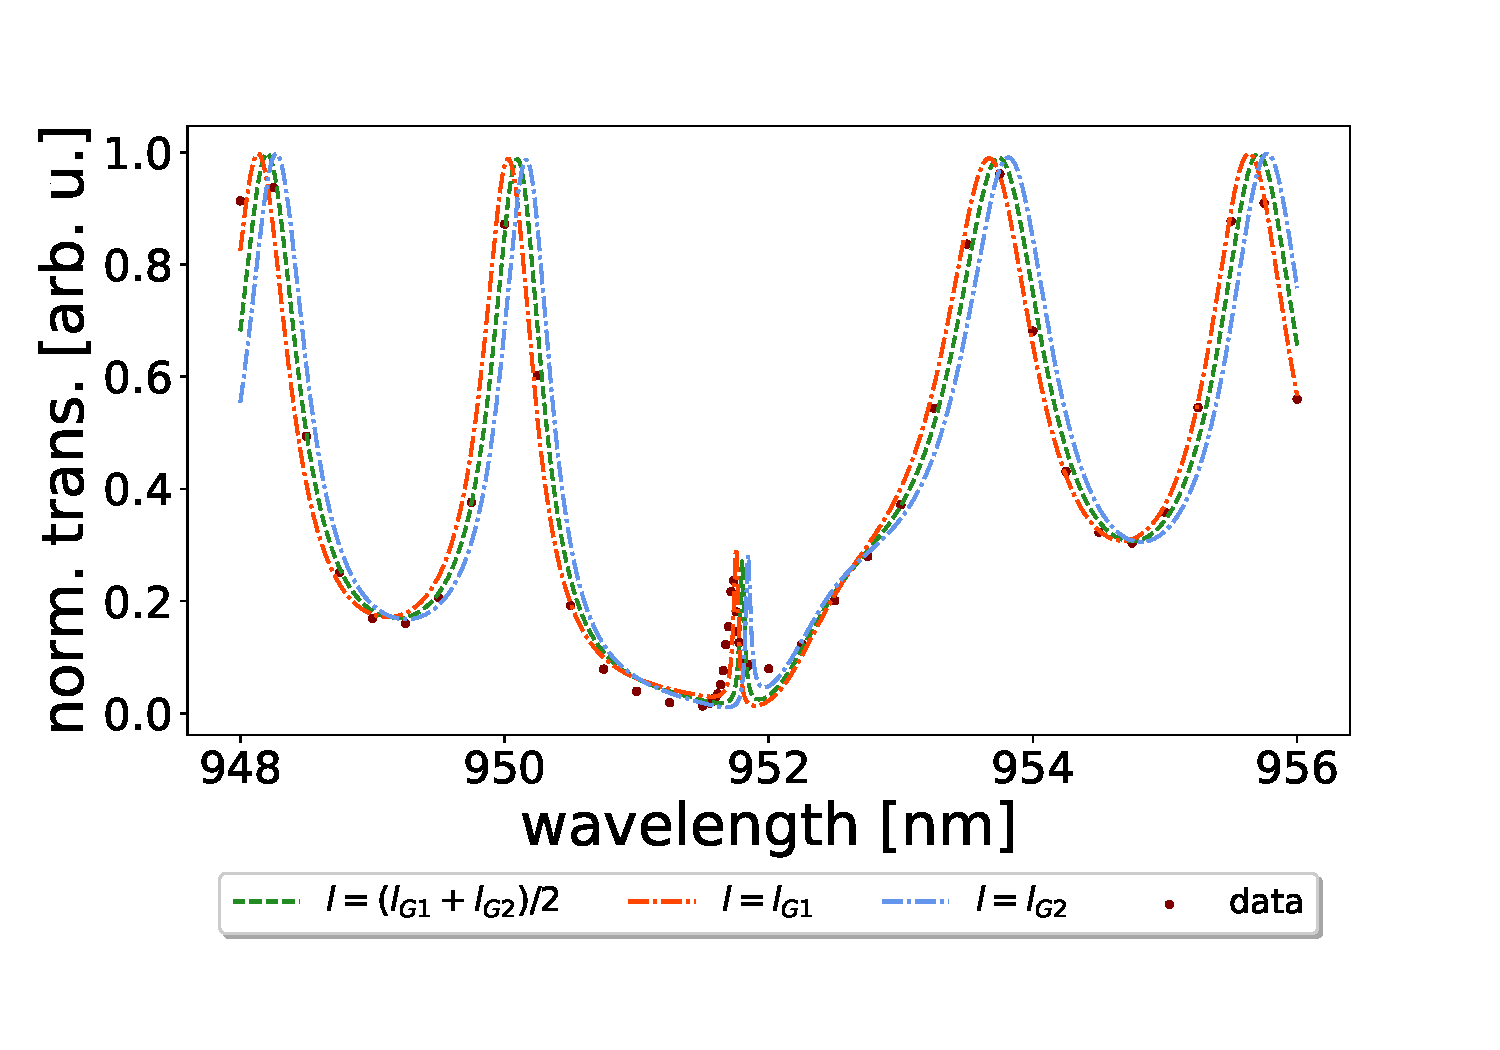
\includegraphics[width=\textwidth]{figures/results/238um_long_scan_sim_comparison.pdf}
        \caption{$l_{G1} = 239.3975 \mu m$, $l_{G2} = 239.4317 \mu m$, $(l_{G1} + l_{G2})/2 = 239.4146 \mu m$}
        \label{fig:238um_long_scan_sim_comparison}
    \end{subfigure}
    \begin{subfigure}[b]{0.49\textwidth}
        \centering
        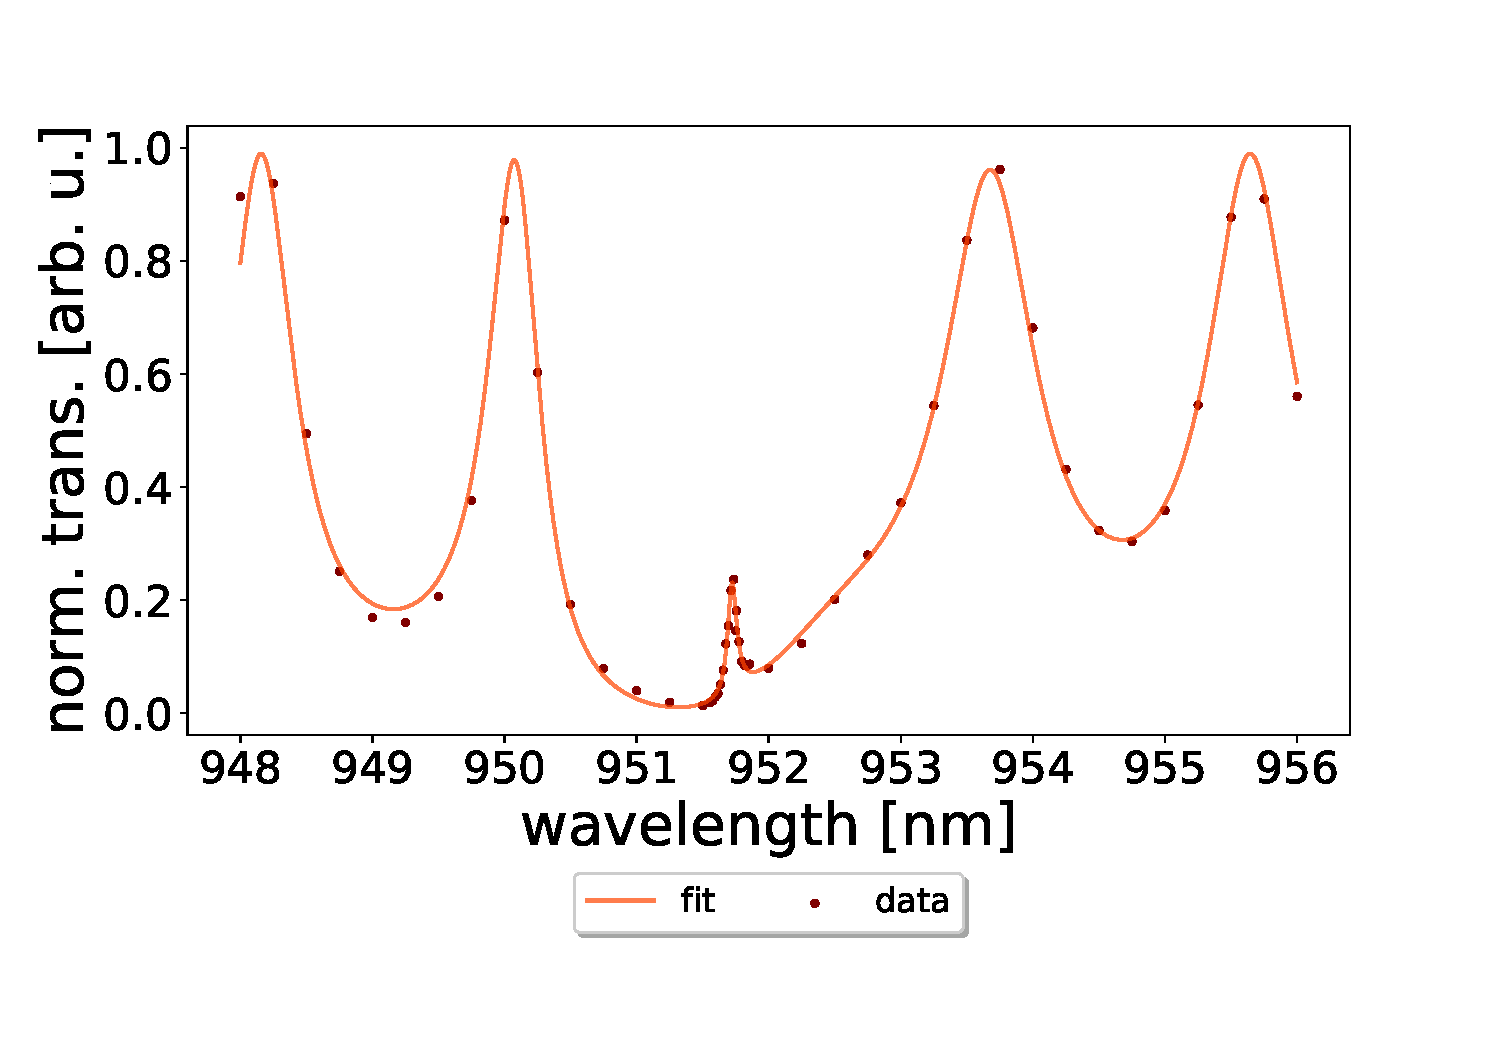
\includegraphics[width=\textwidth]{figures/results/238um_long_scan_fit.pdf}
        \caption{}
        \label{fig:238um_long_scan_fit}
    \end{subfigure}
\end{figure}


Fano mirror \emph{G1} fitting parameters:
\begin{equation}
    \begin{split}
        &\lambda_0 = 951.728 \pm 0.027 \text{nm}, \:\: \lambda_1 = 951.943 \pm 0.0428 \text{nm}, \:\: t_d = 0.823 \pm 0.015, \:\: \\&\gamma_{\lambda} = 0.535 \pm 0.056 \text{nm}, \:\: \beta = 7.788 \cdot 10^{-7} \pm 1.480 \cdot 10^{-7}.
    \end{split}
\end{equation}

Fano mirror \emph{G2} fitting parameters:
\begin{equation}
    \begin{split}
        &\lambda_0 = 951.330 \pm 0.072 \text{nm}, \:\: \lambda_1 = 951.328 \pm 0.110 \text{nm}, \:\: t_d = 0.827 \pm 0.016, \:\: \\&\gamma_{\lambda} = 0.641 \pm 0.131 \text{nm}, \:\: \beta = 1.819 \cdot 10^{-6} \pm 9.314 \cdot 10^{-7}.
    \end{split}
\end{equation}

Cavity parameters:
\begin{equation}
    l = 238.9240 \pm 0.0021 \mu m, \:\: L = 0.0387 \pm 0.0989.
\end{equation}

\begin{figure}[h!]
    \centering
    \begin{subfigure}[b]{0.49\textwidth}
        \centering
        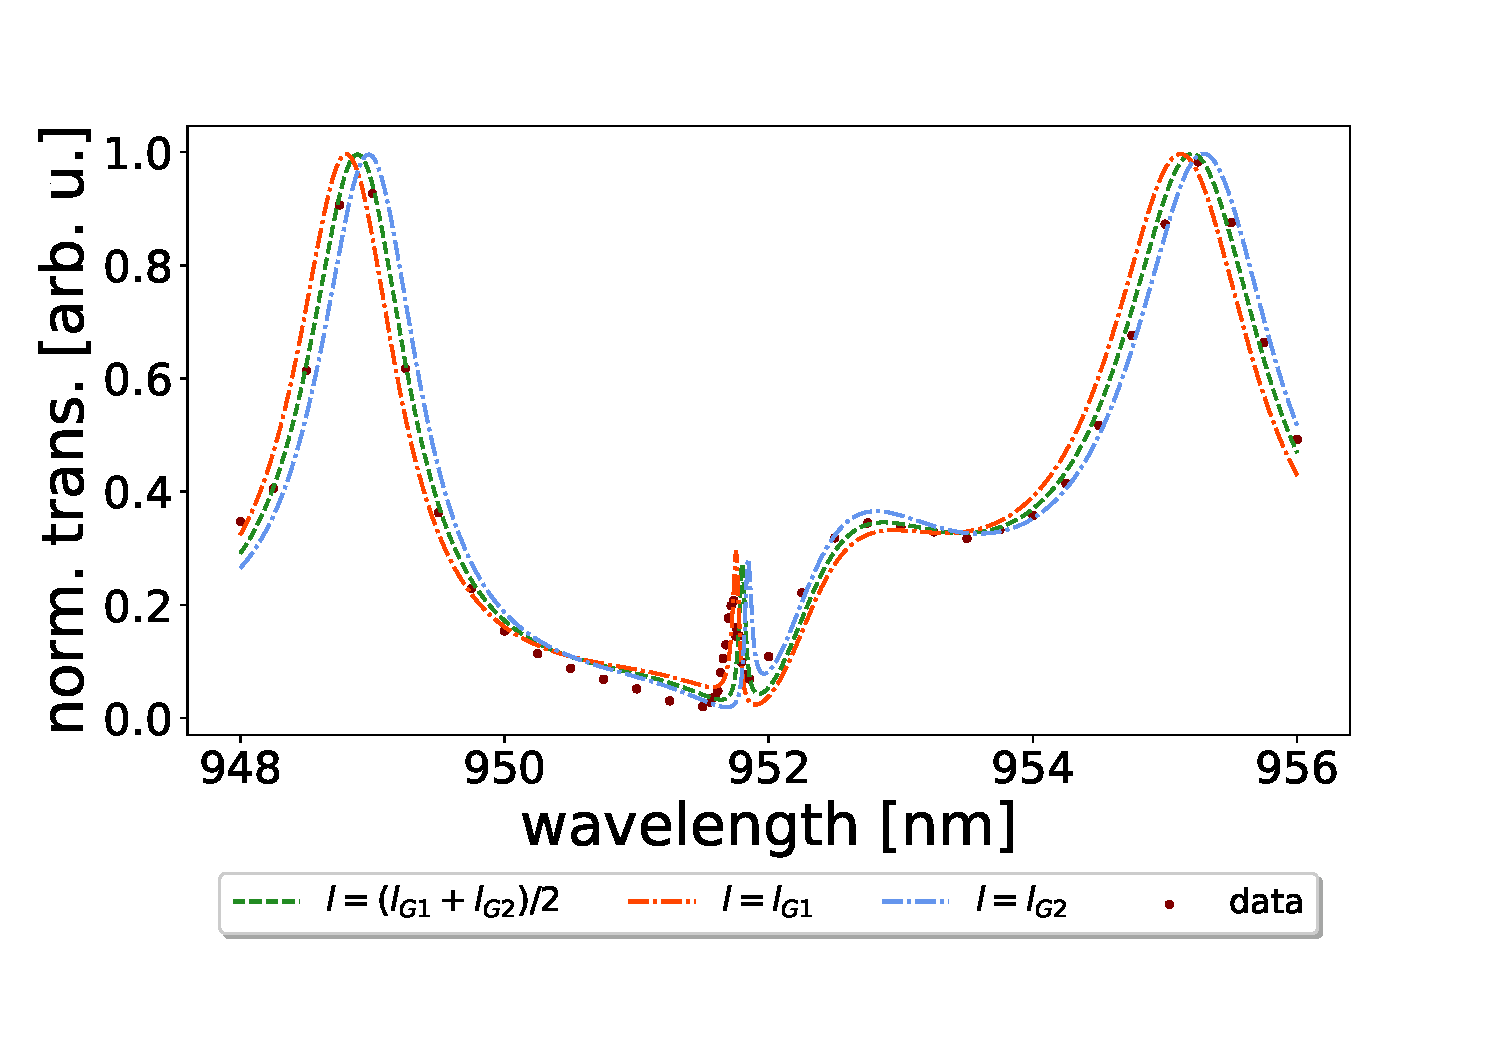
\includegraphics[width=\textwidth]{figures/results/129um_long_scan_sim_comparison.pdf}
        \caption{$l_{G1} = 140.4152 \mu m$, $l_{G2} = 140.4401 \mu m$, $(l_{G1} + l_{G2})/2 = 140.4277 \mu m$}
        \label{fig:129um_long_scan_sim_comparison}
    \end{subfigure}
    \begin{subfigure}[b]{0.49\textwidth}
        \centering
        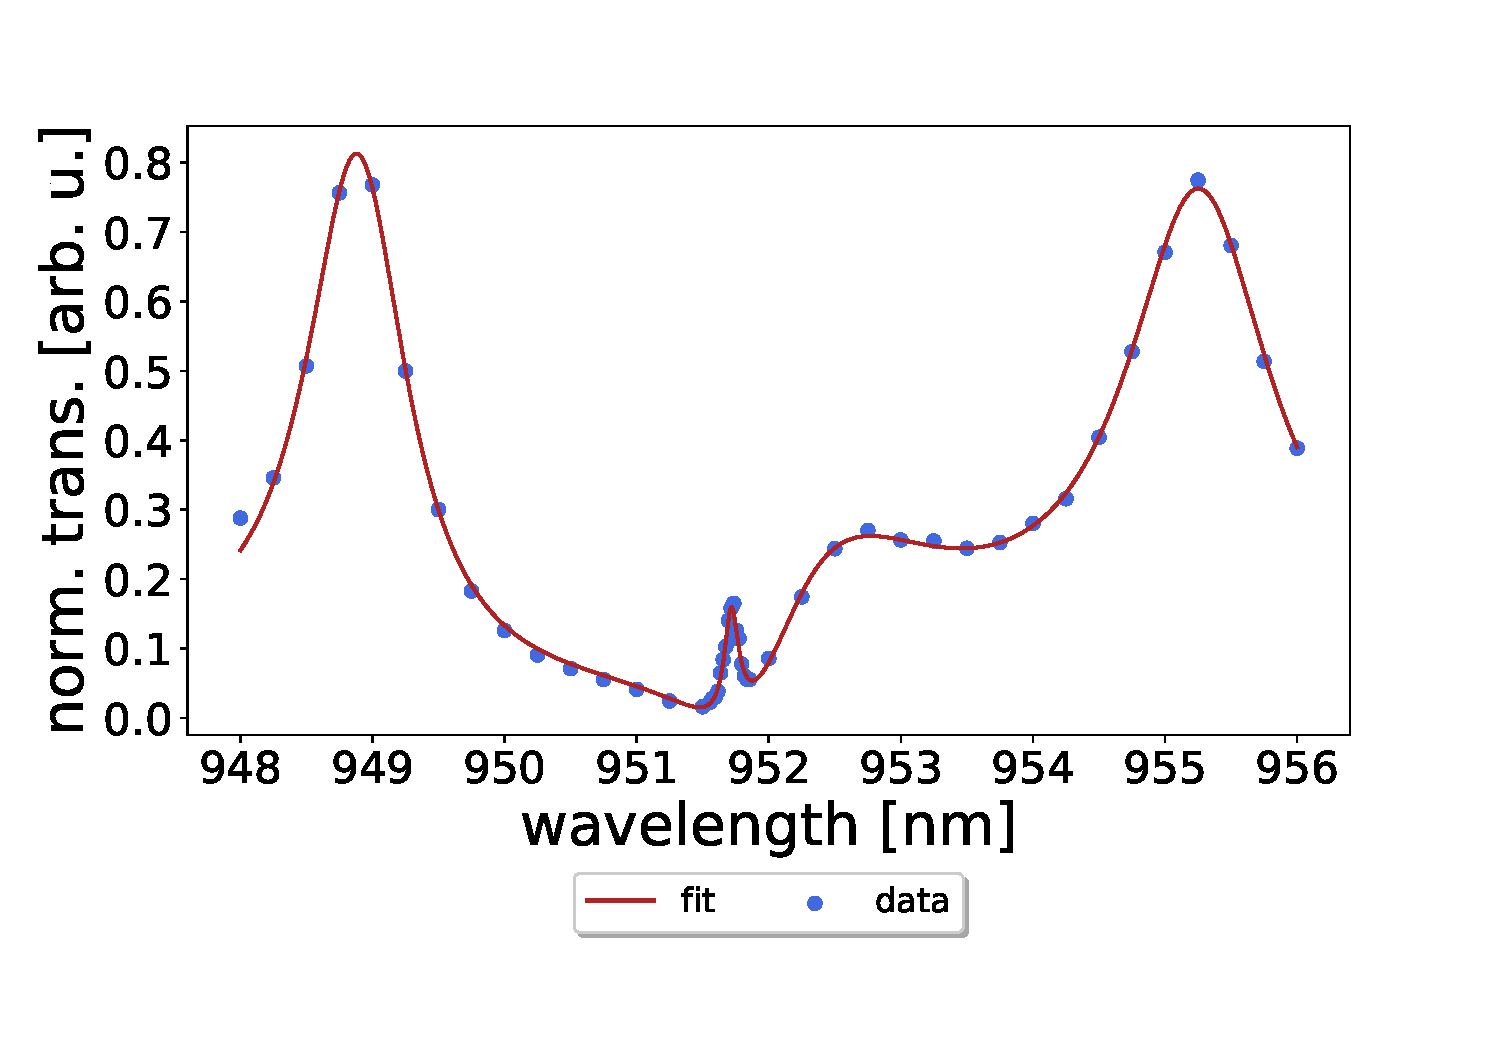
\includegraphics[width=\textwidth]{figures/results/129um_long_scan_fit.pdf}
        \caption{}
        \label{fig:129um_long_scan_fit}
    \end{subfigure}
\end{figure}

Fano mirror \emph{G1} fitting parameters:
\begin{equation}
    \begin{split}
        &\lambda_0 = 951.799 \pm 0.020 \text{nm}, \:\: \lambda_1 = 951.852 \pm 0.0433 \text{nm}, \:\: t_d = 0.816 \pm 0.010, \:\: \\&\gamma_{\lambda} = 0.548 \pm 0.043 \text{nm}, \:\: \beta = 8.335 \cdot 10^{-7} \pm 1.105 \cdot 10^{-7}.
    \end{split}
\end{equation}

Fano mirror \emph{G2} fitting parameters:
\begin{equation}
    \begin{split}
        &\lambda_0 = 951.485 \pm 0.035 \text{nm}, \:\: \lambda_1 = 951.709 \pm 0.036 \text{nm}, \:\: t_d = 0.823 \pm 0.009, \:\: \\&\gamma_{\lambda} = 0.549 \pm 0.039 \text{nm}, \:\: \beta = 1.187 \cdot 10^{-6} \pm 2.810 \cdot 10^{-7}.
    \end{split}
\end{equation}

Cavity parameters:
\begin{equation}
    l = 139.003 \pm 0.001 \mu m, \:\: L = 0.143 \pm 0.037.
\end{equation}

\begin{figure}[h!]
    \centering
    \begin{subfigure}[b]{0.49\textwidth}
        \centering
        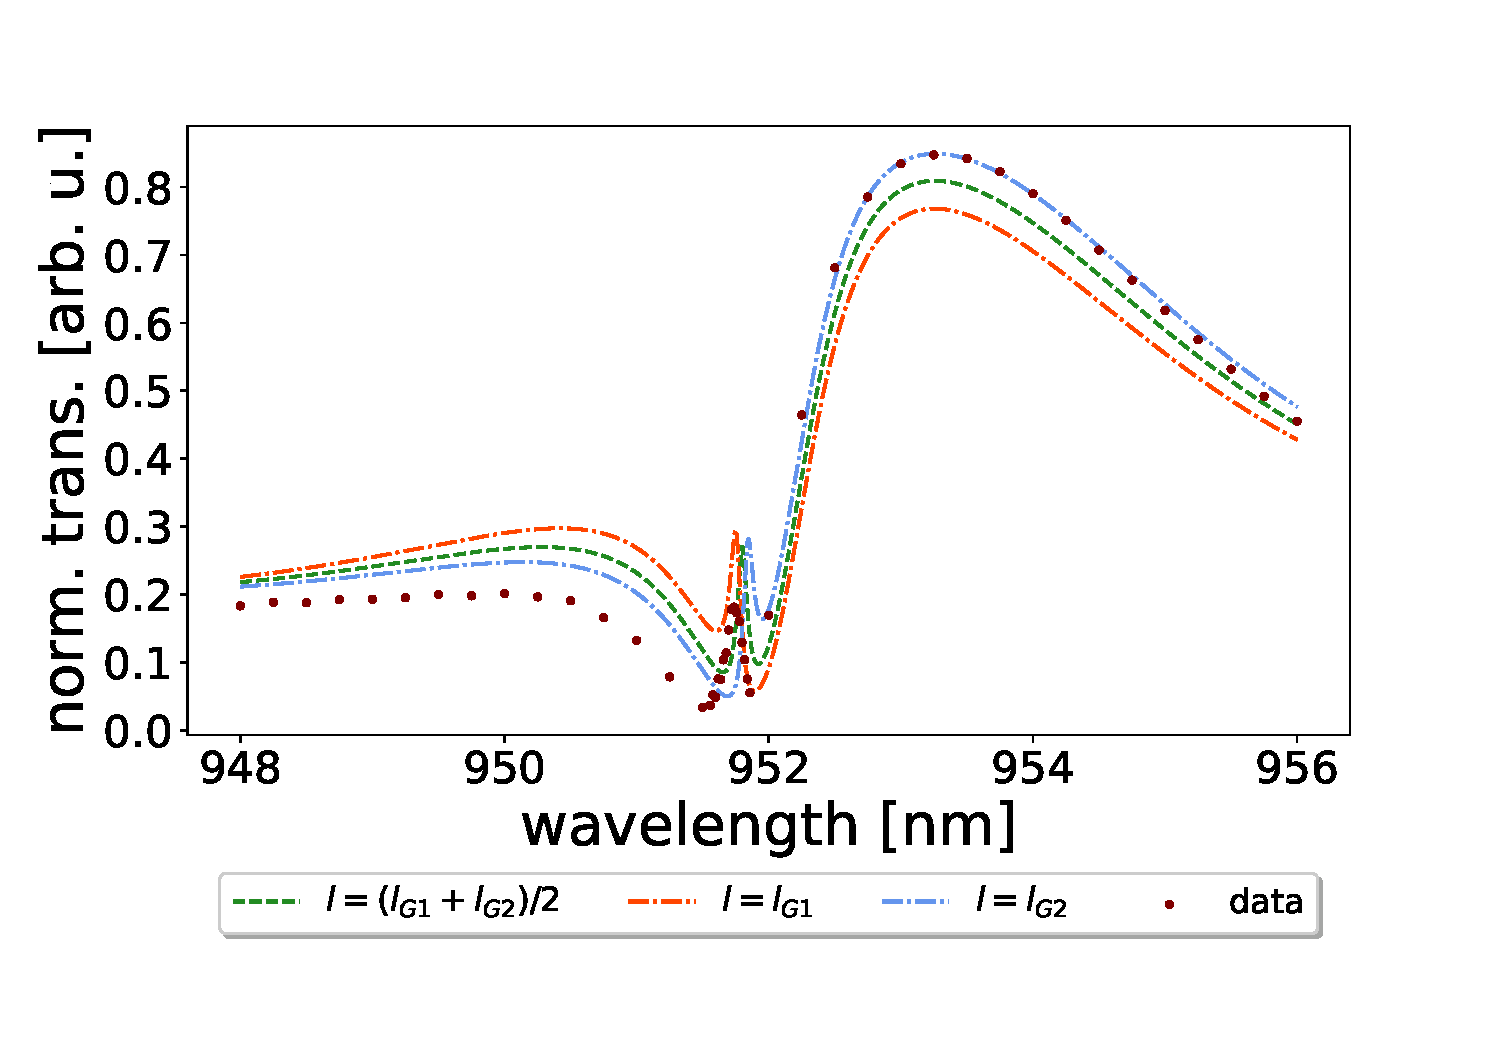
\includegraphics[width=\textwidth]{figures/results/34um_long_scan_sim_comparison.pdf}
        \caption{}
        \label{fig:34um_long_scan_sim_comparison}
    \end{subfigure}
    \begin{subfigure}[b]{0.49\textwidth}
        \centering
        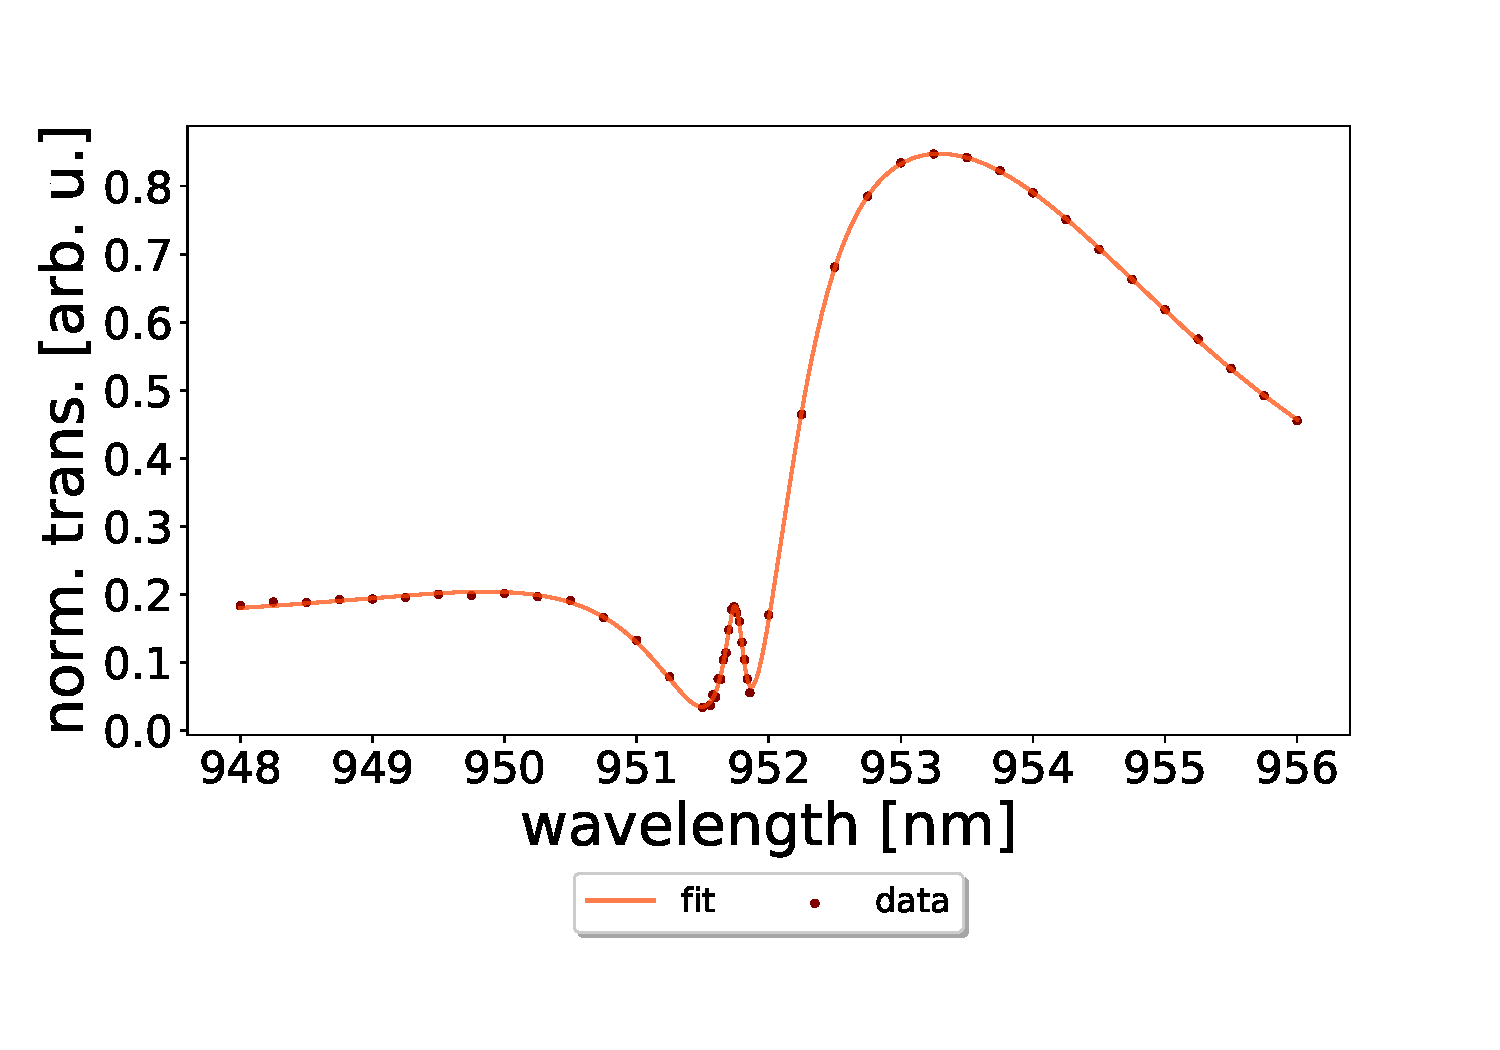
\includegraphics[width=\textwidth]{figures/results/34um_long_scan_fit.pdf}
        \caption{}
        \label{fig:34um_long_scan_fit}
    \end{subfigure}
\end{figure}


\subsubsection{Double fano off-resonance Fabry-Perot cavity}

Figures:
\begin{itemize}
    \item Off-resonance double fano transmission as a function of wavelength (show that the off resonance transmission goes close to 100 percent for a well-aligned cavity).
\end{itemize}

\subsubsection{The double fano linewidth}

\begin{figure}[h!]
    \centering
    \begin{subfigure}[b]{0.49\textwidth}
        \centering
        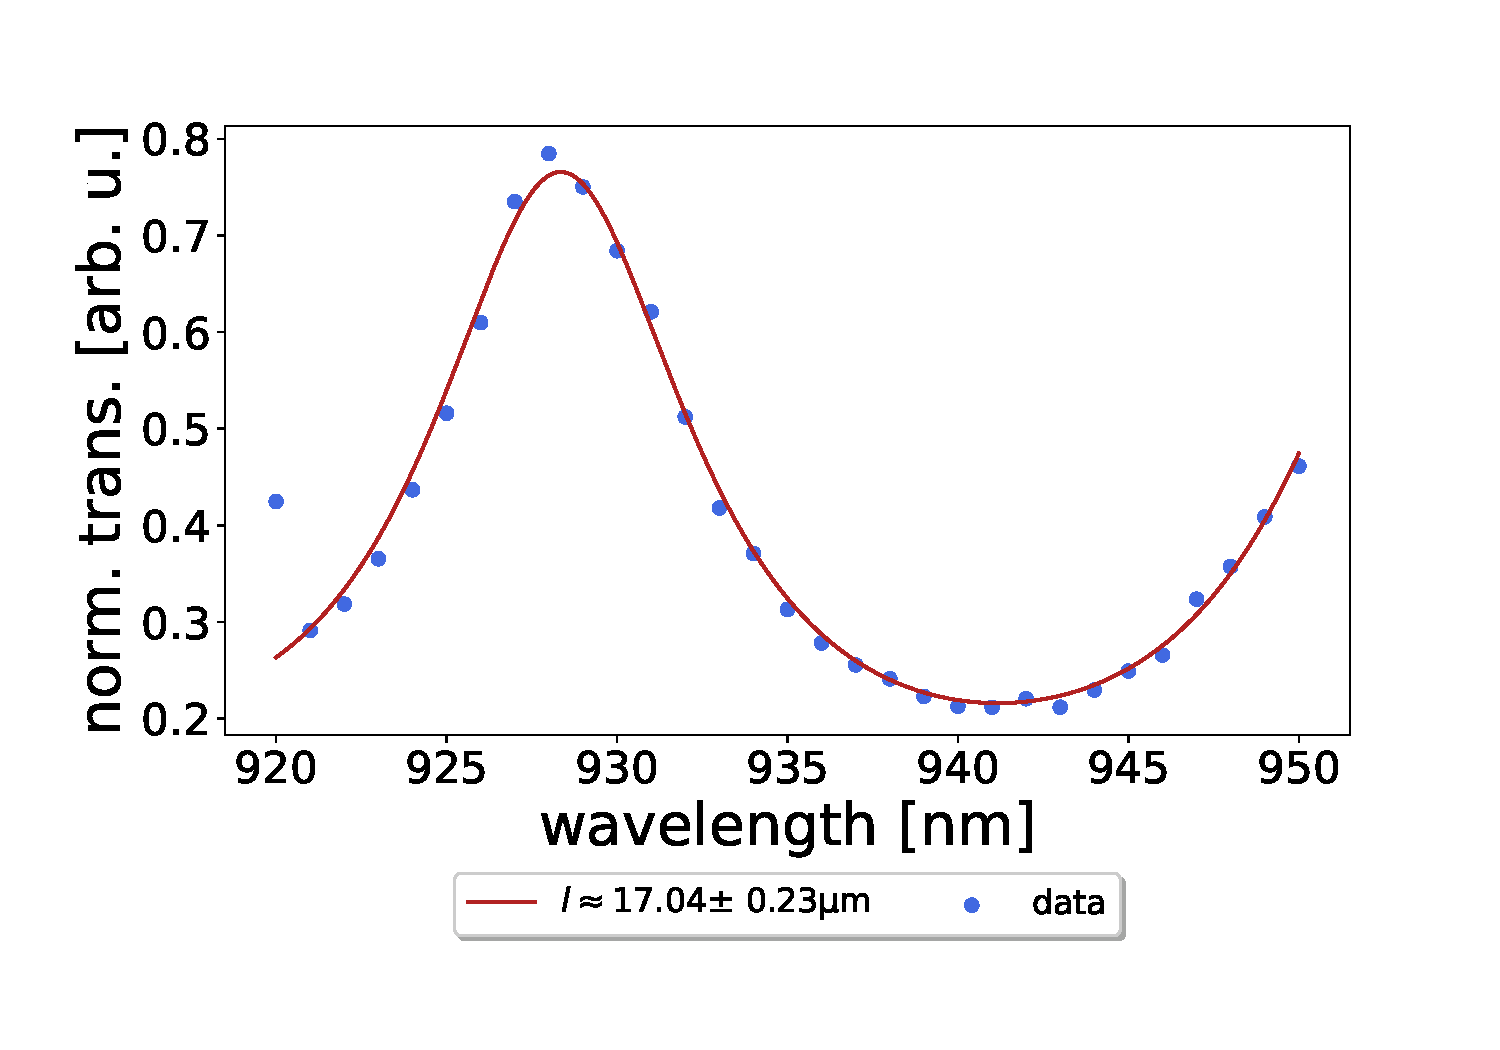
\includegraphics[width=\textwidth]{figures/results/double fano fits/30um_M3:M5_FSR_scan.pdf}
        \caption{}
        \label{fig:short_double_fano_FSR}
    \end{subfigure}
    \begin{subfigure}[b]{0.49\textwidth}
        \centering
        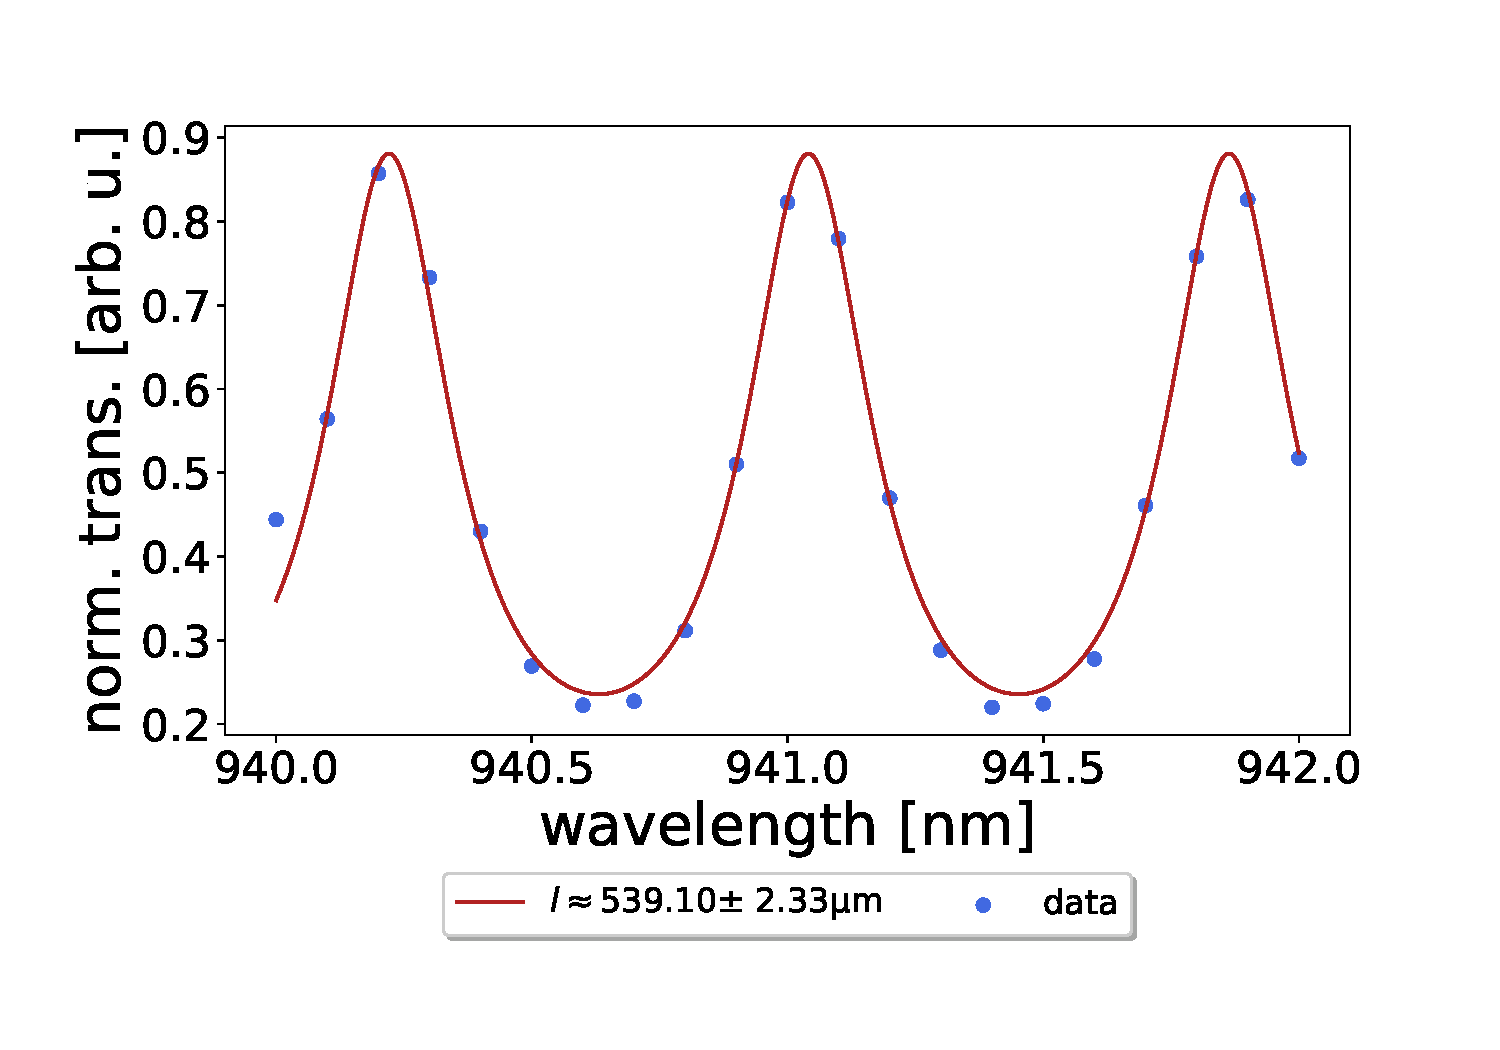
\includegraphics[width=\textwidth]{figures/results/double fano fits/550um_M3:M5_FSR_scan.pdf}
        \caption{}
        \label{fig:long_double_fano_FSR}
    \end{subfigure}
\end{figure}

\begin{figure}[h!]
    \centering
    \begin{subfigure}[b]{0.49\textwidth}
        \centering
        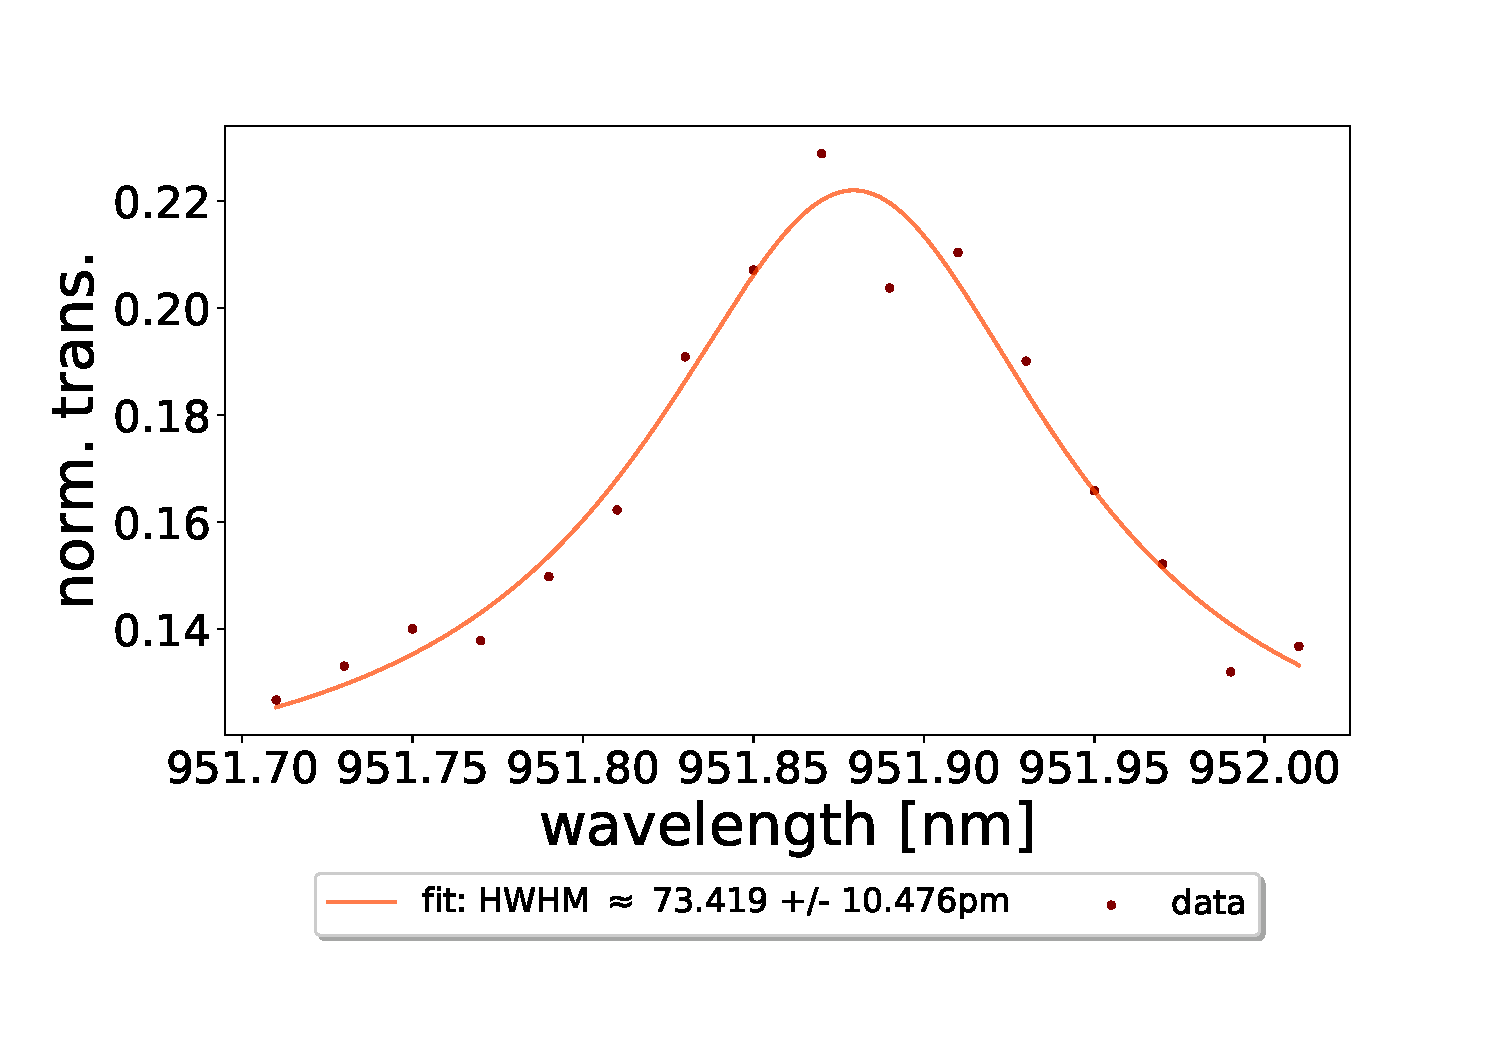
\includegraphics[width=\textwidth]{figures/results/double fano fits/30um_M3:M5_fit_4.pdf}
        \caption{}
        \label{fig:short_double_fano_trans}
    \end{subfigure}
    \begin{subfigure}[b]{0.49\textwidth}
        \centering
        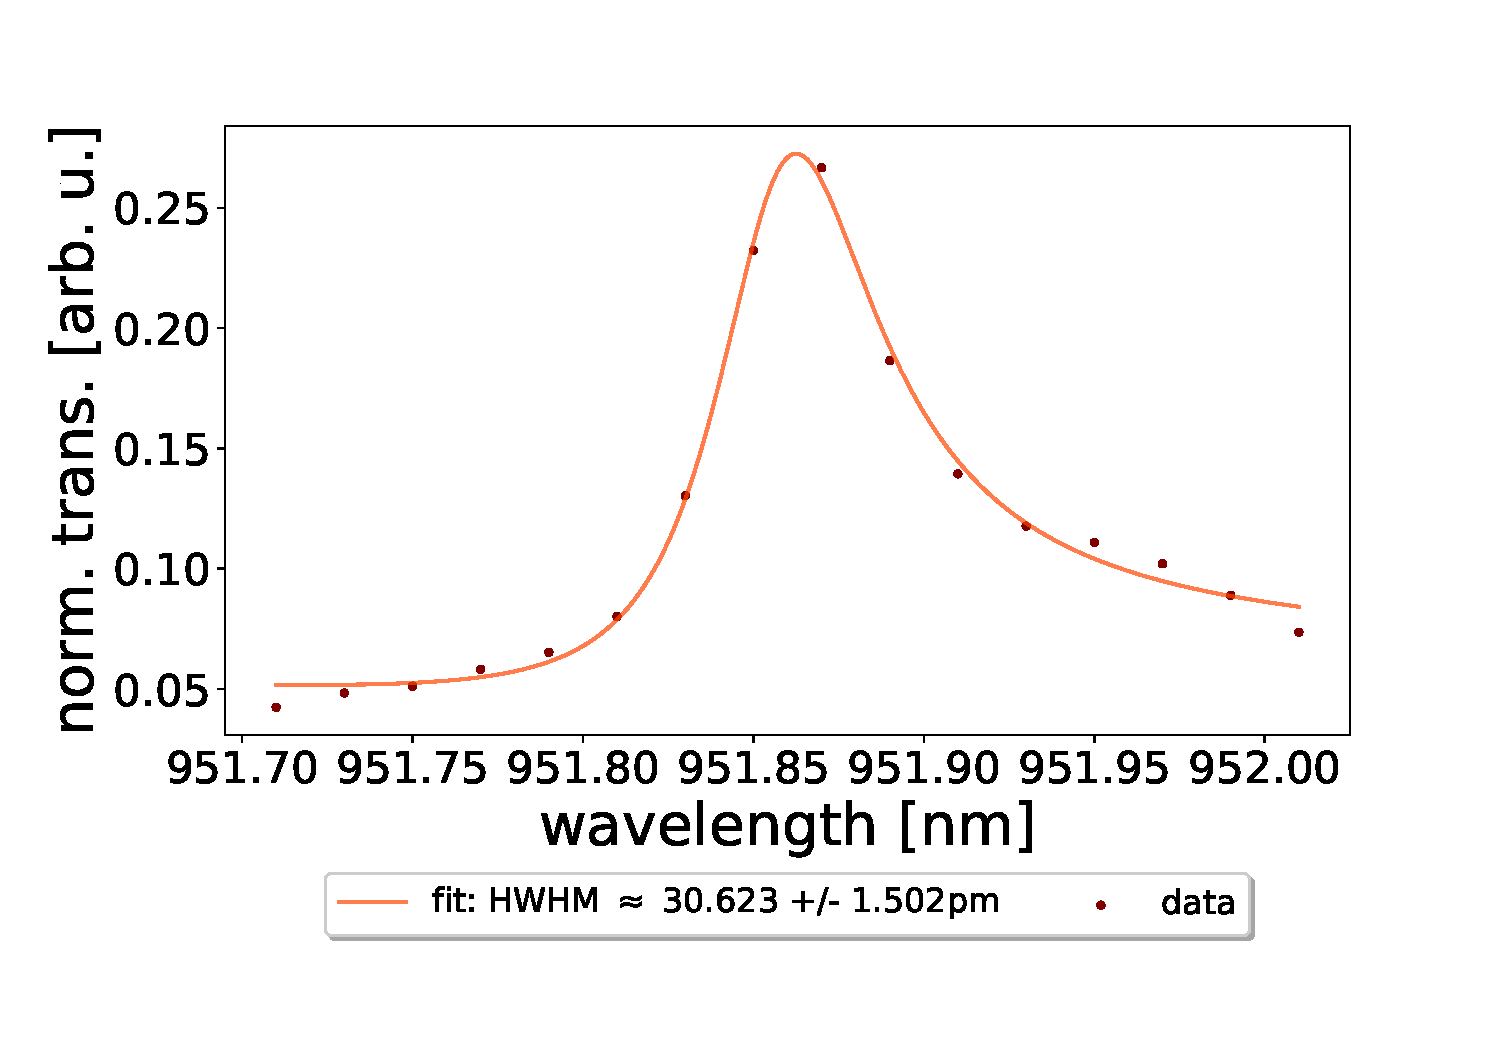
\includegraphics[width=\textwidth]{figures/results/double fano fits/550um_M3:M5_fit_1.pdf}
        \caption{}
        \label{fig:long_double_fano_trans}
    \end{subfigure}
\end{figure}

Measurement 1:

\begin{figure}[h!]
    \centering
    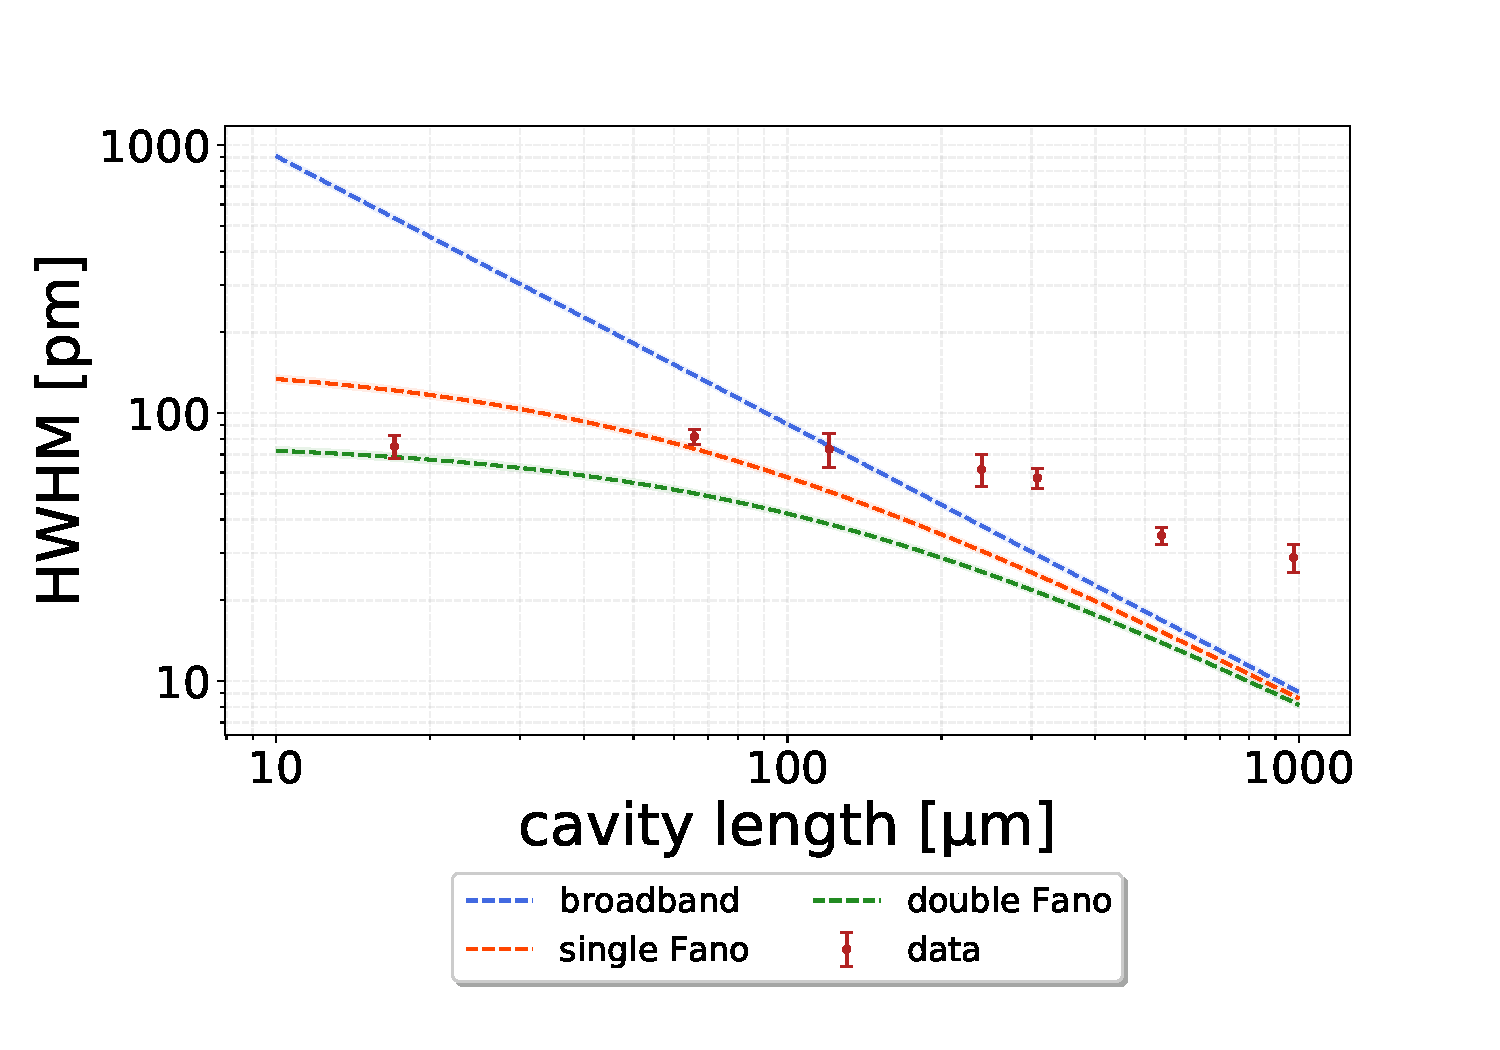
\includegraphics[width=0.7\textwidth]{figures/results/double fano fits/HWHM_vs_cavity_length_result_1st_measurement_only.pdf}
    \caption{}
    \label{fig:HWHM_vs_l_double_fano_result_1st}
\end{figure}

Measurement 2: 

\begin{figure}[h!]
    \centering
    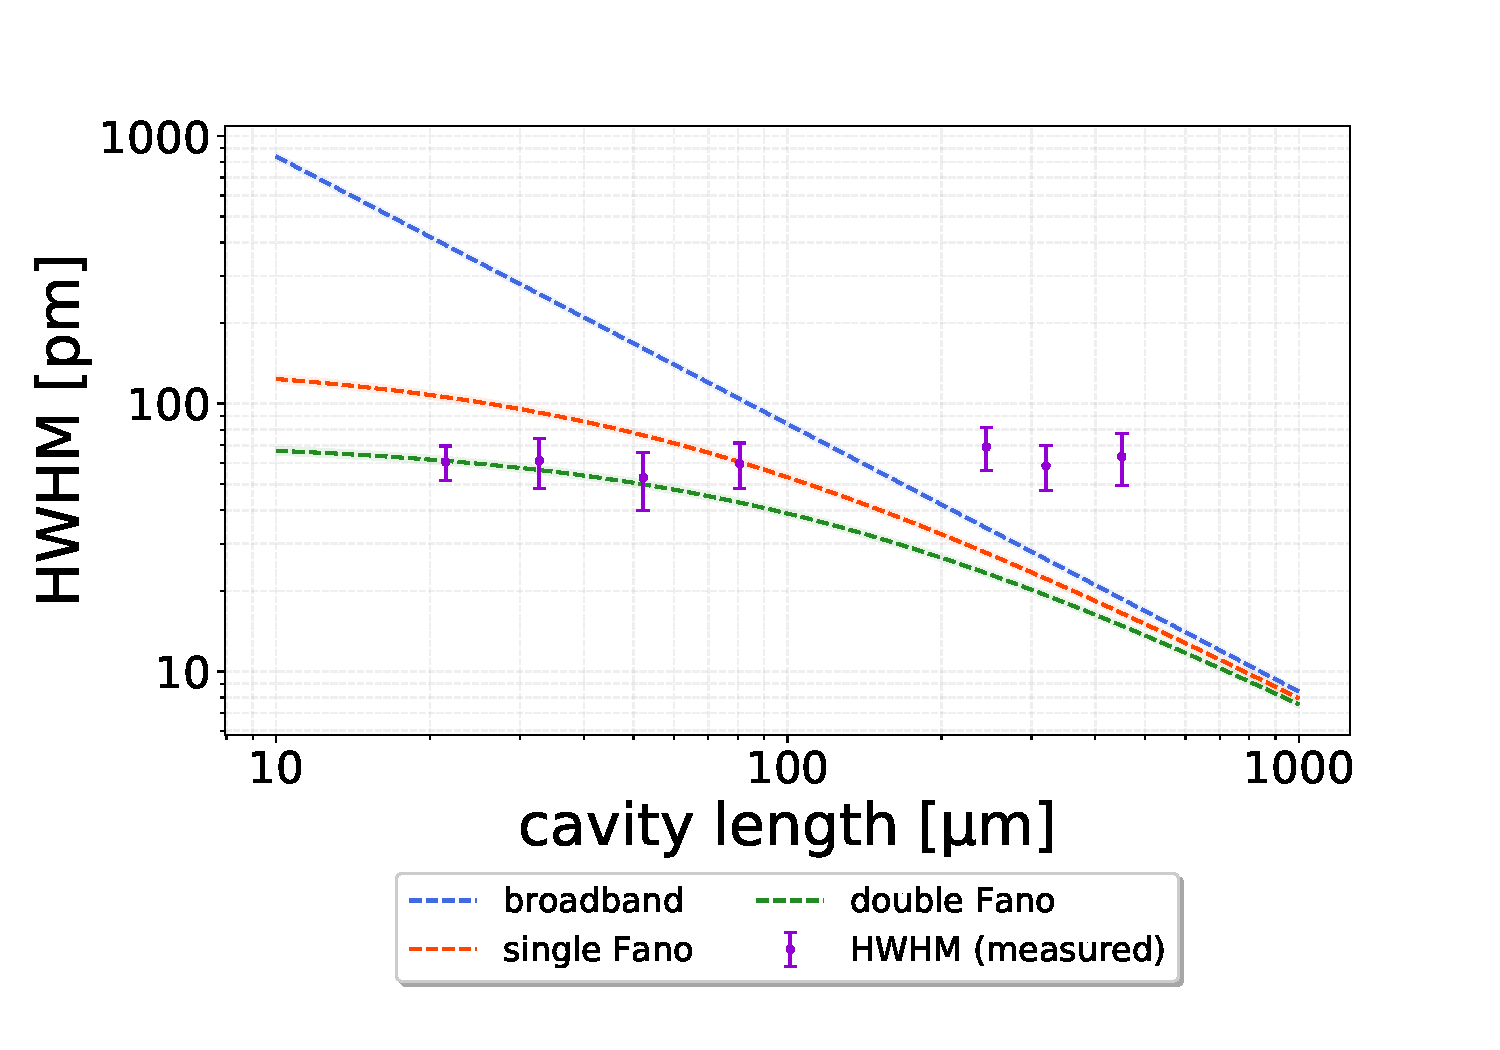
\includegraphics[width=0.7\textwidth]{figures/results/double fano fits/HWHM_vs_cavity_length_result_2nd_measurement_only.pdf}
    \caption{}
    \label{fig:HWHM_vs_l_double_fano_result_2nd}
\end{figure}

Average of the two measurements: 
\begin{figure}[h!]
    \centering
    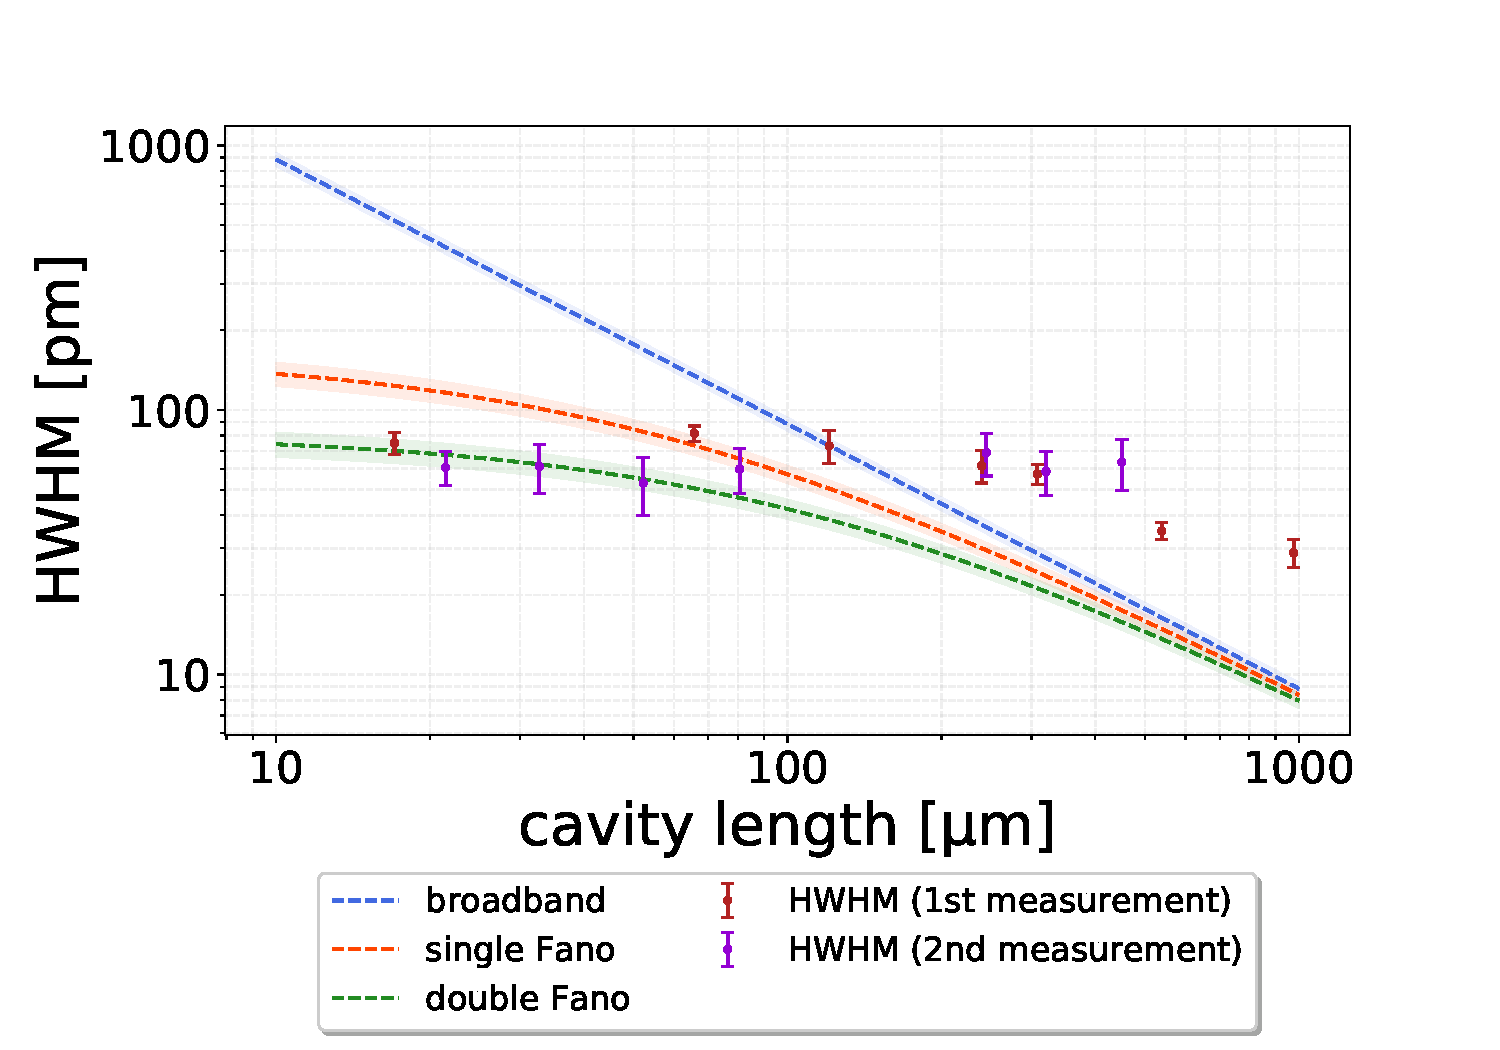
\includegraphics[width=0.7\textwidth]{figures/results/double fano fits/HWHM_vs_cavity_length_result.pdf}
    \caption{}
    \label{fig:HWHM_vs_l_double_fano_result}
\end{figure}

Figures: 
\begin{itemize}
    \item "Semi-short" scan data, fit to the double fano transmission model. 
    \item Short scan data, fit to the Fano function (for measuring linewidth).
    \item Linewidth as a function of cavity length (compare double fano, single fano and broadband cavitites).
\end{itemize}

